\documentclass{extbook}[14pt]
\usepackage{multicol, enumerate, enumitem, hyperref, color, soul, setspace, parskip, fancyhdr, amssymb, amsthm, amsmath, latexsym, units, mathtools}
\everymath{\displaystyle}
\usepackage[headsep=0.5cm,headheight=0cm, left=1 in,right= 1 in,top= 1 in,bottom= 1 in]{geometry}
\usepackage{dashrule}  % Package to use the command below to create lines between items
\newcommand{\litem}[1]{\item #1

\rule{\textwidth}{0.4pt}}
\pagestyle{fancy}
\lhead{}
\chead{Answer Key for Progress Quiz 6 Version A}
\rhead{}
\lfoot{9689-6866}
\cfoot{}
\rfoot{Spring 2021}
\begin{document}
\textbf{This key should allow you to understand why you choose the option you did (beyond just getting a question right or wrong). \href{https://xronos.clas.ufl.edu/mac1105spring2020/courseDescriptionAndMisc/Exams/LearningFromResults}{More instructions on how to use this key can be found here}.}

\textbf{If you have a suggestion to make the keys better, \href{https://forms.gle/CZkbZmPbC9XALEE88}{please fill out the short survey here}.}

\textit{Note: This key is auto-generated and may contain issues and/or errors. The keys are reviewed after each exam to ensure grading is done accurately. If there are issues (like duplicate options), they are noted in the offline gradebook. The keys are a work-in-progress to give students as many resources to improve as possible.}

\rule{\textwidth}{0.4pt}

\begin{enumerate}\litem{
Solve the rational equation below. Then, choose the interval(s) that the solution(s) belongs to.
\[ \frac{2x}{-4x -4} + \frac{-4x^{2}}{16x^{2} +24 x + 8} = \frac{4}{-4x -2} \]The solution is \( \text{There are two solutions: } x = -0.758 \text{ and } x = 1.758 \), which is option E.\begin{enumerate}[label=\Alph*.]
\item \( x_1 \in [-1.15, -0.74] \text{ and } x_2 \in [-1.4,0.7] \)


\item \( x \in [1.36,1.93] \)


\item \( \text{All solutions lead to invalid or complex values in the equation.} \)


\item \( x \in [-0.58,-0.05] \)


\item \( x_1 \in [-1.15, -0.74] \text{ and } x_2 \in [0.7,3.3] \)

* $x = -0.758 \text{ and } x = 1.758$, which is the correct option.
\end{enumerate}

\textbf{General Comment:} Distractors are different based on the number of solutions. Remember that after solving, we need to make sure our solution does not make the original equation divide by zero!
}
\litem{
Determine the domain of the function below.
\[ f(x) = \frac{6}{12x^{2} +21 x + 9} \]The solution is \( \text{All Real numbers except } x = -1.000 \text{ and } x = -0.750. \), which is option C.\begin{enumerate}[label=\Alph*.]
\item \( \text{All Real numbers.} \)

This corresponds to thinking the denominator has complex roots or that rational functions have a domain of all Real numbers.
\item \( \text{All Real numbers except } x = a, \text{ where } a \in [-12, -12] \)

All Real numbers except $x = -12.000$, which corresponds to removing a distractor value from the denominator.
\item \( \text{All Real numbers except } x = a \text{ and } x = b, \text{ where } a \in [-1.04, -0.83] \text{ and } b \in [-0.88, -0.66] \)

All Real numbers except $x = -1.000$ and $x = -0.750$, which is the correct option.
\item \( \text{All Real numbers except } x = a \text{ and } x = b, \text{ where } a \in [-12, -12] \text{ and } b \in [-9.1, -8.84] \)

All Real numbers except $x = -12.000$ and $x = -9.000$, which corresponds to not factoring the denominator correctly.
\item \( \text{All Real numbers except } x = a, \text{ where } a \in [-1.04, -0.83] \)

All Real numbers except $x = -1.000$, which corresponds to removing only 1 value from the denominator.
\end{enumerate}

\textbf{General Comment:} Recall that dividing by zero is not a real number. Therefore the domain is all real numbers \textbf{except} those that make the denominator 0.
}
\litem{
Choose the graph of the equation below.
\[ f(x) = \frac{1}{x + 2} - 3 \]The solution is the graph below, which is option C.
\begin{center}
    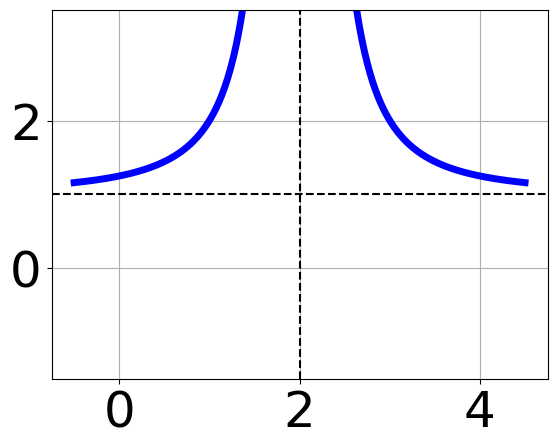
\includegraphics[width=0.3\textwidth]{../Figures/rationalEquationToGraphCA.png}
\end{center}\begin{enumerate}[label=\Alph*.]
\begin{multicols}{2}
\item 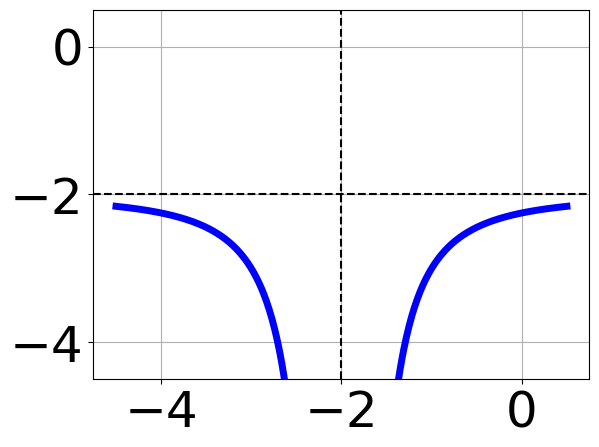
\includegraphics[width = 0.3\textwidth]{../Figures/rationalEquationToGraphAA.png}
\item 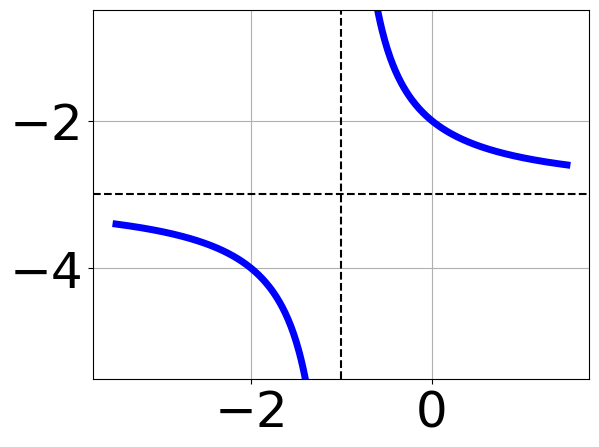
\includegraphics[width = 0.3\textwidth]{../Figures/rationalEquationToGraphBA.png}
\item 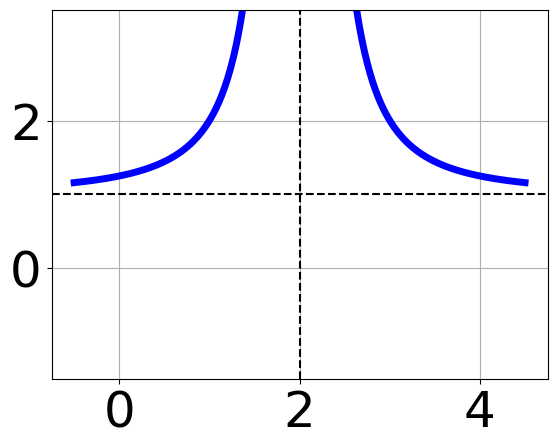
\includegraphics[width = 0.3\textwidth]{../Figures/rationalEquationToGraphCA.png}
\item 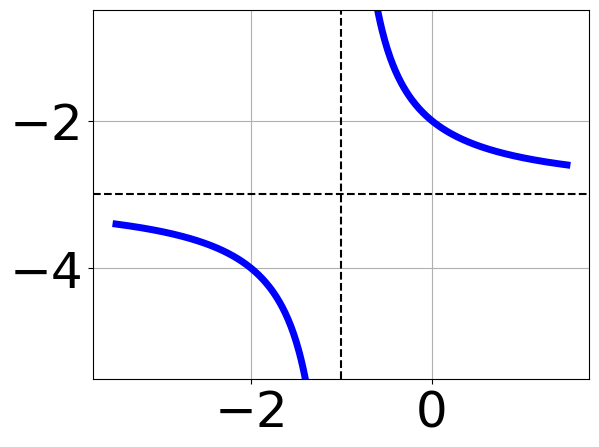
\includegraphics[width = 0.3\textwidth]{../Figures/rationalEquationToGraphDA.png}
\end{multicols}\item None of the above.\end{enumerate}
\textbf{General Comment:} Remember that the general form of a basic rational equation is $ f(x) = \frac{a}{(x-h)^n} + k$, where $a$ is the leading coefficient (and in this case, we assume is either $1$ or $-1$), $n$ is the degree (in this case, either $1$ or $2$), and $(h, k)$ is the intersection of the asymptotes.
}
\litem{
Choose the graph of the equation below.
\[ f(x) = \frac{-1}{x + 2} - 3 \]The solution is the graph below, which is option A.
\begin{center}
    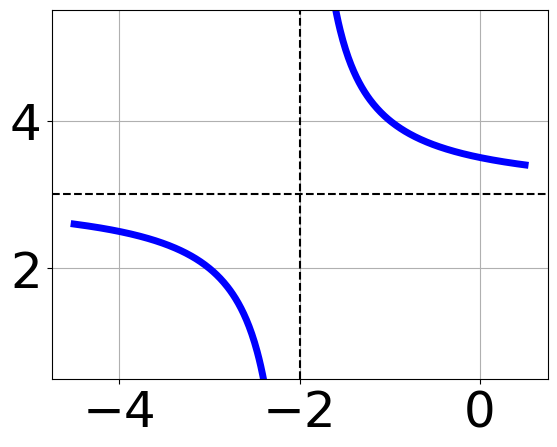
\includegraphics[width=0.3\textwidth]{../Figures/rationalEquationToGraphCopyAA.png}
\end{center}\begin{enumerate}[label=\Alph*.]
\begin{multicols}{2}
\item 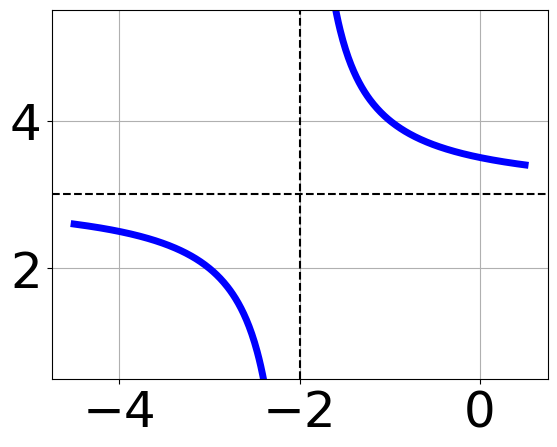
\includegraphics[width = 0.3\textwidth]{../Figures/rationalEquationToGraphCopyAA.png}
\item 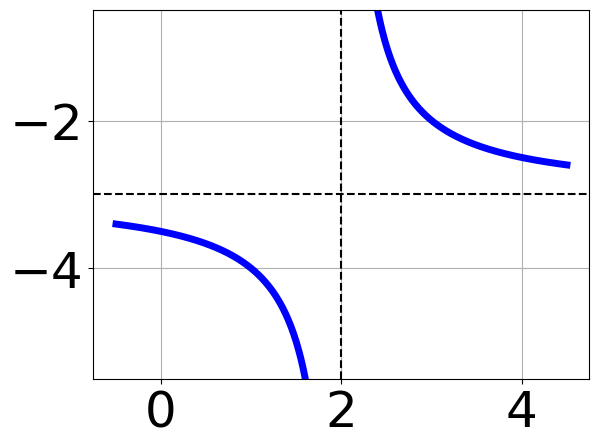
\includegraphics[width = 0.3\textwidth]{../Figures/rationalEquationToGraphCopyBA.png}
\item 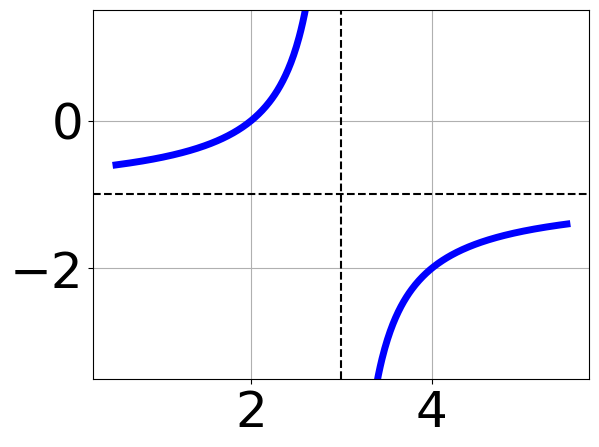
\includegraphics[width = 0.3\textwidth]{../Figures/rationalEquationToGraphCopyCA.png}
\item 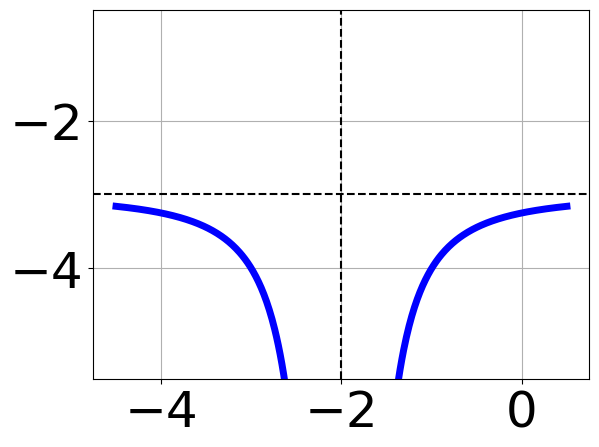
\includegraphics[width = 0.3\textwidth]{../Figures/rationalEquationToGraphCopyDA.png}
\end{multicols}\item None of the above.\end{enumerate}
\textbf{General Comment:} Remember that the general form of a basic rational equation is $ f(x) = \frac{a}{(x-h)^n} + k$, where $a$ is the leading coefficient (and in this case, we assume is either $1$ or $-1$), $n$ is the degree (in this case, either $1$ or $2$), and $(h, k)$ is the intersection of the asymptotes.
}
\litem{
Choose the equation of the function graphed below.

\begin{center}
    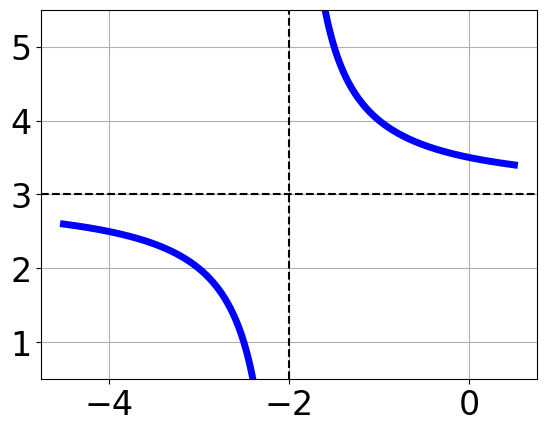
\includegraphics[width=0.5\textwidth]{../Figures/rationalGraphToEquationA.png}
\end{center}


The solution is \( f(x) = \frac{1}{x + 2} + 2 \), which is option C.\begin{enumerate}[label=\Alph*.]
\item \( f(x) = \frac{-1}{x - 2} + 2 \)

Corresponds to using the general form $f(x) = \frac{a}{x+h}+k$ and the opposite leading coefficient.
\item \( f(x) = \frac{1}{(x + 2)^2} + 2 \)

Corresponds to thinking the graph was a shifted version of $\frac{1}{x^2}$.
\item \( f(x) = \frac{1}{x + 2} + 2 \)

This is the correct option.
\item \( f(x) = \frac{-1}{(x - 2)^2} + 2 \)

Corresponds to thinking the graph was a shifted version of $\frac{1}{x^2}$, using the general form $f(x) = \frac{a}{x+h}+k$, and the opposite leading coefficient.
\item \( \text{None of the above} \)

This corresponds to believing the vertex of the graph was not correct.
\end{enumerate}

\textbf{General Comment:} Remember that the general form of a basic rational equation is $ f(x) = \frac{a}{(x-h)^n} + k$, where $a$ is the leading coefficient (and in this case, we assume is either $1$ or $-1$), $n$ is the degree (in this case, either $1$ or $2$), and $(h, k)$ is the intersection of the asymptotes.
}
\litem{
Choose the equation of the function graphed below.

\begin{center}
    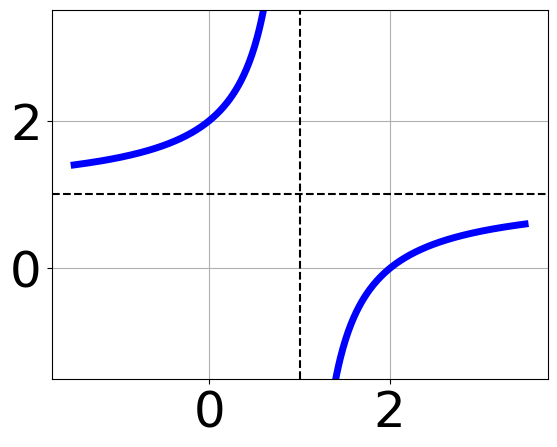
\includegraphics[width=0.5\textwidth]{../Figures/rationalGraphToEquationCopyA.png}
\end{center}


The solution is \( f(x) = \frac{1}{x - 3} + 2 \), which is option D.\begin{enumerate}[label=\Alph*.]
\item \( f(x) = \frac{-1}{x + 3} + 2 \)

Corresponds to using the general form $f(x) = \frac{a}{x+h}+k$ and the opposite leading coefficient.
\item \( f(x) = \frac{1}{(x - 3)^2} + 2 \)

Corresponds to thinking the graph was a shifted version of $\frac{1}{x^2}$.
\item \( f(x) = \frac{-1}{(x + 3)^2} + 2 \)

Corresponds to thinking the graph was a shifted version of $\frac{1}{x^2}$, using the general form $f(x) = \frac{a}{x+h}+k$, and the opposite leading coefficient.
\item \( f(x) = \frac{1}{x - 3} + 2 \)

This is the correct option.
\item \( \text{None of the above} \)

This corresponds to believing the vertex of the graph was not correct.
\end{enumerate}

\textbf{General Comment:} Remember that the general form of a basic rational equation is $ f(x) = \frac{a}{(x-h)^n} + k$, where $a$ is the leading coefficient (and in this case, we assume is either $1$ or $-1$), $n$ is the degree (in this case, either $1$ or $2$), and $(h, k)$ is the intersection of the asymptotes.
}
\litem{
Solve the rational equation below. Then, choose the interval(s) that the solution(s) belongs to.
\[ \frac{5}{-3x + 2} + 5 = \frac{-2}{18x -12} \]The solution is \( x = 0.978 \), which is option C.\begin{enumerate}[label=\Alph*.]
\item \( x_1 \in [0, 2] \text{ and } x_2 \in [1.02,1.19] \)

$x = 0.978 \text{ and } x = 1.133$, which corresponds to getting the correct solution and believing there should be a second solution to the equation.
\item \( x_1 \in [-1.5, 0.8] \text{ and } x_2 \in [0.93,1.09] \)

$x = -0.356 \text{ and } x = 0.978$, which corresponds to getting the correct solution and believing there should be a second solution to the equation.
\item \( x \in [0.98,1.98] \)

* $x = 0.978$, which is the correct option.
\item \( \text{All solutions lead to invalid or complex values in the equation.} \)

This corresponds to thinking $x = 0.978$ leads to dividing by zero in the original equation, which it does not.
\item \( x \in [-1.5,0.8] \)

$x = -0.356$, which corresponds to not distributing the factor $-3x + 2$ correctly when trying to eliminate the fraction.
\end{enumerate}

\textbf{General Comment:} Distractors are different based on the number of solutions. Remember that after solving, we need to make sure our solution does not make the original equation divide by zero!
}
\litem{
Solve the rational equation below. Then, choose the interval(s) that the solution(s) belongs to.
\[ \frac{-21}{28x + 35} + 1 = \frac{-21}{28x + 35} \]The solution is \( \text{all solutions are invalid or lead to complex values in the equation.} \), which is option C.\begin{enumerate}[label=\Alph*.]
\item \( x_1 \in [-1.25, 0.75] \text{ and } x_2 \in [-3.25,-0.25] \)

$x = -1.250 \text{ and } x = -1.250$, which corresponds to getting the correct solution and believing there should be a second solution to the equation.
\item \( x \in [-1.25,-0.25] \)

$x = -1.250$, which corresponds to not checking if this value leads to dividing by 0 in the original equation and thus is not a valid solution.
\item \( \text{All solutions lead to invalid or complex values in the equation.} \)

*$x = -1.250$ leads to dividing by 0 in the original equation and thus is not a valid solution, which is the correct option.
\item \( x \in [1.25,4.25] \)

$x = 1.250$, which corresponds to not distributing the factor $28x + 35$ correctly when trying to eliminate the fraction.
\item \( x_1 \in [-1.25, 0.75] \text{ and } x_2 \in [0.25,2.25] \)

$x = -1.250 \text{ and } x = 1.250$, which corresponds to getting the correct solution and believing there should be a second solution to the equation.
\end{enumerate}

\textbf{General Comment:} Distractors are different based on the number of solutions. Remember that after solving, we need to make sure our solution does not make the original equation divide by zero!
}
\litem{
Solve the rational equation below. Then, choose the interval(s) that the solution(s) belongs to.
\[ \frac{-5x}{-3x -7} + \frac{-6x^{2}}{21x^{2} +55 x + 14} = \frac{-3}{-7x -2} \]The solution is \( \text{There are two solutions: } x = 0.834 \text{ and } x = -0.868 \), which is option E.\begin{enumerate}[label=\Alph*.]
\item \( x \in [-0.68,0.07] \)


\item \( x_1 \in [0.27, 1.06] \text{ and } x_2 \in [-4,-1.6] \)


\item \( \text{All solutions lead to invalid or complex values in the equation.} \)


\item \( x \in [-0.88,-0.63] \)


\item \( x_1 \in [0.27, 1.06] \text{ and } x_2 \in [-1.2,-0.8] \)

* $x = 0.834 \text{ and } x = -0.868$, which is the correct option.
\end{enumerate}

\textbf{General Comment:} Distractors are different based on the number of solutions. Remember that after solving, we need to make sure our solution does not make the original equation divide by zero!
}
\litem{
Determine the domain of the function below.
\[ f(x) = \frac{5}{36x^{2} +6 x -30} \]The solution is \( \text{All Real numbers except } x = -1.000 \text{ and } x = 0.833. \), which is option C.\begin{enumerate}[label=\Alph*.]
\item \( \text{All Real numbers except } x = a \text{ and } x = b, \text{ where } a \in [-36.1, -35.8] \text{ and } b \in [29.5, 30.3] \)

All Real numbers except $x = -36.000$ and $x = 30.000$, which corresponds to not factoring the denominator correctly.
\item \( \text{All Real numbers except } x = a, \text{ where } a \in [-36.1, -35.8] \)

All Real numbers except $x = -36.000$, which corresponds to removing a distractor value from the denominator.
\item \( \text{All Real numbers except } x = a \text{ and } x = b, \text{ where } a \in [-1.3, -0.3] \text{ and } b \in [-0.3, 1.8] \)

All Real numbers except $x = -1.000$ and $x = 0.833$, which is the correct option.
\item \( \text{All Real numbers.} \)

This corresponds to thinking the denominator has complex roots or that rational functions have a domain of all Real numbers.
\item \( \text{All Real numbers except } x = a, \text{ where } a \in [-1.3, -0.3] \)

All Real numbers except $x = -1.000$, which corresponds to removing only 1 value from the denominator.
\end{enumerate}

\textbf{General Comment:} Recall that dividing by zero is not a real number. Therefore the domain is all real numbers \textbf{except} those that make the denominator 0.
}
\end{enumerate}

\end{document}